\documentclass[../probability-notes.tex]{subfiles}
\begin{document}
    %%%%%%%%%%%%%%%%%%%%%%%%%%%%%%%%%%%%%%%%%%%%%%%%%%%%%%%%%%%%%%%%%%%%%%%%%%%
    \section{Gamma Distribution}
    A random variable is said to have a Gamma distribution if for parameters $(\alpha, \lambda)$ with $\lambda > 0, \alpha > 0$, it has the following probability distribution
    \begin{align*}
        p_{X}(x) = \begin{cases}
            \frac{\lambda e^{-\lambda x} (\lambda x)^{\alpha - 1}}{\Gamma(\alpha)} &\mbox{if $x \geq 0$}\\
            0 &\mbox{otherwise}
        \end{cases}
    \end{align*}
    The denominator in the above fomula acts as nothing but a normalization constant and is defined as
    \begin{align*}
        \Gamma (\alpha) &= \int_{0}^{\infty} e^{-x} x^{\alpha - 1}\\
        &= (\alpha - 1) \int_{0}^{\infty} e^{-x} x^{\alpha - 2} dy \:\text{using integration by parts}\\
        &= (\alpha - 1) \Gamma (\alpha - 1)
    \end{align*}

    Note that at $\alpha = 1$, $\Gamma (1) = \int_{0}^{\infty} e^{-x} = 1$. Hence, if $\alpha$ is an integer, $\Gamma(\alpha) = (\alpha-1) !$ using the recursion relation derived above.\newline

    For a fixed $\lambda$, as the value of $\alpha$ becomes large, the distribution takes the form of a normal distribution.

    \begin{figure}[h]
    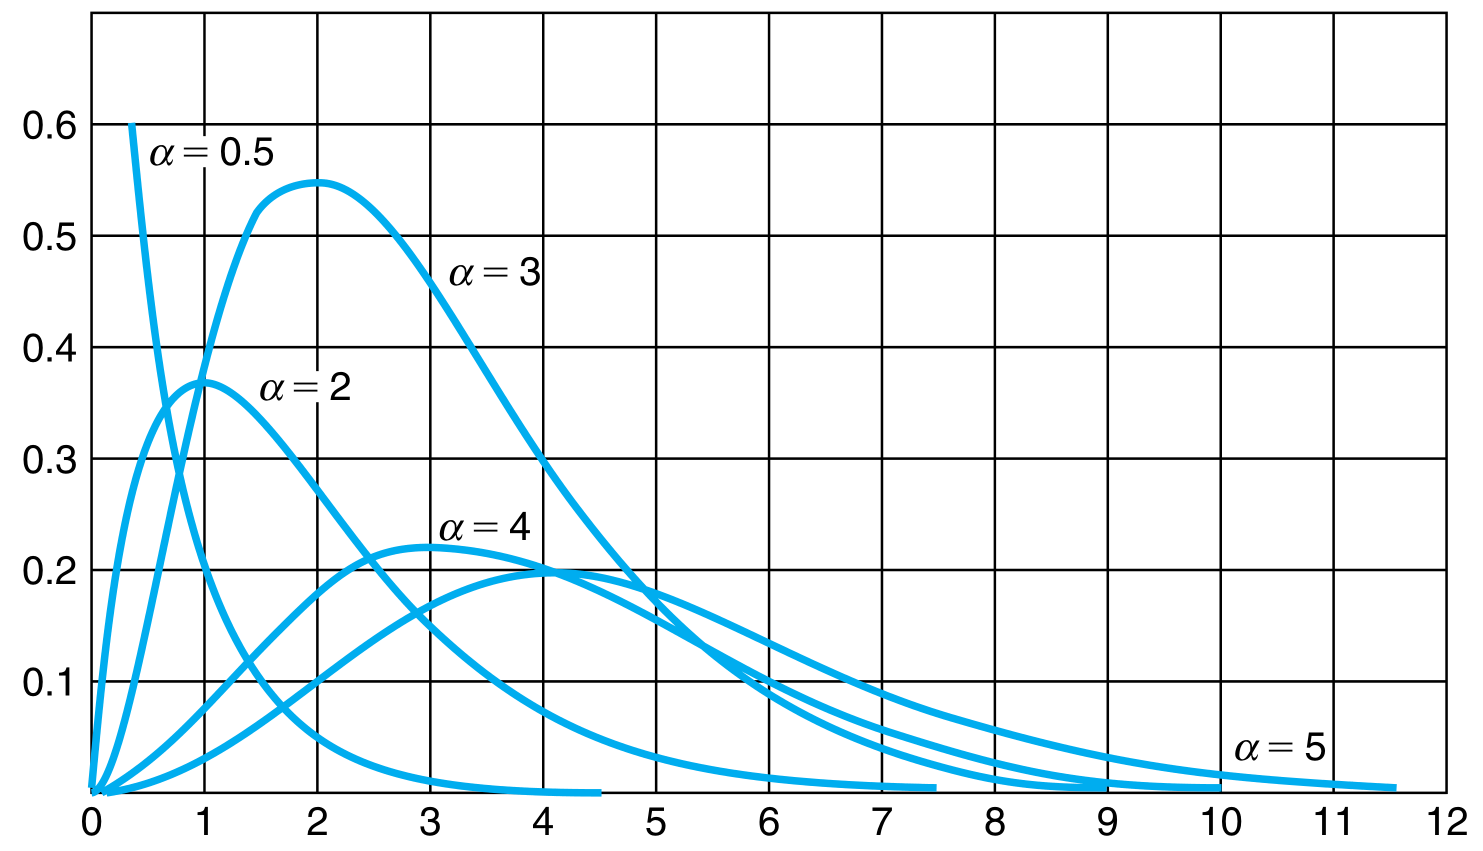
\includegraphics[scale=0.25]{gamma_1}
    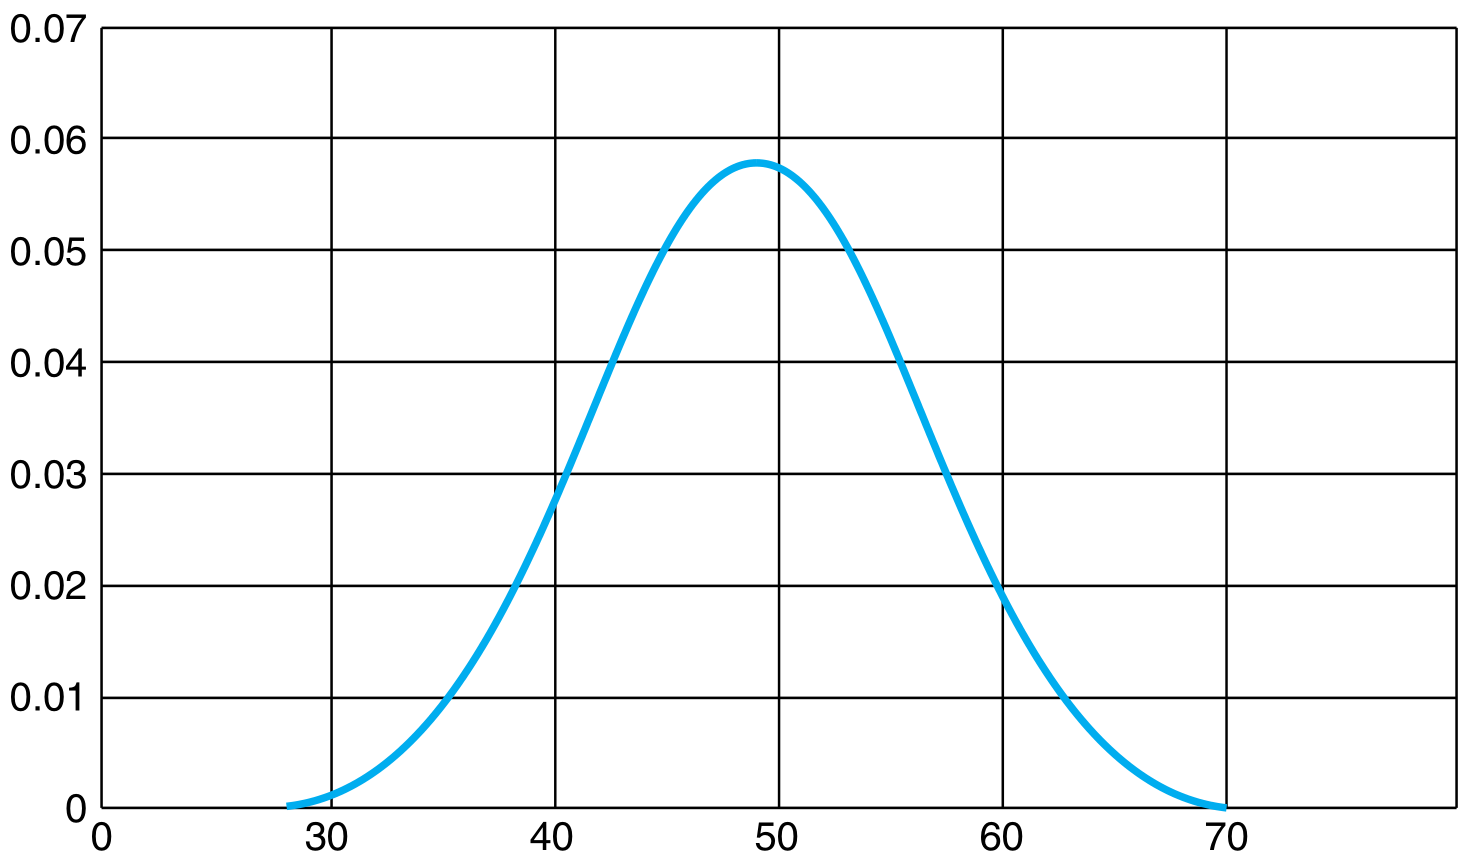
\includegraphics[scale=0.25]{gamma_2}
    \centering
    \caption{Gamma distribution for $\lambda = 1$ and different values of $\alpha$. The second figure shows the distribution for $\alpha = 50$.}
    \label{fig:gamma_1} %\ref{fig:gamma_1}
    \end{figure}

    %%%%%%%%%%%%%%%%%%%%%%%%%%%%%%%%%%%%%%%%%%%%%%%%%%%%%%%%%%%%%%%%%%%%%%%%%%%
    \subsection{Mean, Variance and Moment Generating Function}
    Mean and variance are easily obtainable for this using the moment generating function. Recall
    \begin{align*}
        \phi(t) &= E[e^{tX}]\\
        \phi^{n}(t) &= E[X^{n}]
    \end{align*}

    For the current distribution,
    \begin{align*}
        \phi(t) &= \frac{\lambda^{\alpha}}{\Gamma(\alpha)} \int_{0}^{\infty} e^{tx} e^{-\lambda x} x^{\alpha - 1} dx\\
        &= \bigg(\frac{\lambda}{\lambda - t}\bigg)^{\alpha}
    \end{align*}
    by rearranging the terms to complete an integral of a Gamma distribution with parameters $(\alpha, \lambda - t)$. Differentiating,
    \begin{align*}
        \phi^{\prime}(t) &= \frac{\alpha \lambda^{\alpha}}{(\lambda - t)^{\alpha + 1}}\\
        \phi^{\prime \prime}(t) &= \frac{\alpha(\alpha + 1)\lambda^{\alpha}}{(\lambda - t)^{\alpha + 2}}\\
        \Aboxed{E[X] &= \phi^{\prime}(0) = \frac{\alpha}{\lambda}}\\
        \Aboxed{Var(X) &= \phi^{\prime \prime}(0) = \frac{\alpha}{\lambda^{2}}}
    \end{align*}

    %%%%%%%%%%%%%%%%%%%%%%%%%%%%%%%%%%%%%%%%%%%%%%%%%%%%%%%%%%%%%%%%%%%%%%%%%%%
    \subsection{Sum of Gamma Distributions}
    Let $X_{1}, X_{2}, \ldots, X_{n}$ be $n$ independent random variables that are gamma distributed with parameters \newline$(\alpha_{1}, \lambda), (\alpha_{2}, \lambda), \ldots, (\alpha_{n}, \lambda)$. Then the distribution of the sum of these random variables is itself a gamma distribution with the parameters $\alpha^{\prime} = \sum_{i=1}^{n} \alpha_{i}$ and $\lambda^{\prime} = \lambda$.\newline

    This follows from the moment generating function of the sum of variables
    \begin{align*}
        E[e^{t(X_{1} + \cdots + X_{n})}] &= \prod_{i=1}^{n} E[e^{tX_{i}}] \; \text{by independence}\\
        &= \prod_{i=1}^{n} \bigg(\frac{\lambda}{\lambda - t}\bigg)^{\alpha} = \bigg(\frac{\lambda}{\lambda - t}\bigg)^{\sum_{i=1}^{n} \alpha_{i}}
    \end{align*}
    which is the moment generating function of $Gamma(\sum_{i=1}^{n} \alpha_{i}, \lambda)$.

    %%%%%%%%%%%%%%%%%%%%%%%%%%%%%%%%%%%%%%%%%%%%%%%%%%%%%%%%%%%%%%%%%%%%%%%%%%%
    \subsection{Relation with Exponential Distribution}
    With $\alpha = 1$, the Gamma distribution becomes an Exponential distribution with parameter $\lambda$. Based on the previous theorem, the sum of $n$ independent Gamma distributed random variables with parameters $(1, \lambda)$ or equivalently, $n$ independent Exponentially distributed random variables with parameter $\lambda$ is a Gamma distribution with parameters $(n, \lambda)$.
\end{document}
